\section{Projected results}\label{sec_countrate}
A GPD-based event generator for DVCS-BH on a deuterium target was run, assuming a luminosity of $3/20\cdot 10^{35}$ cm$^2$ s$^{-1}$ (where the factor $3/20$ accounts for the ratio of polarized neutrons to the total nucleons in ND$_3$) and a beam time of 100 days. The output of the generator was fed to the CLAS12 Fast-MC code, which included acceptance and resolution effects for CLAS12 and the CND. An additional factor of $10\%$ was also applied to mimick the efficiency of the CND for neutrons\footnote{Actually, this factor was adopted globally for ALL neutrons, even those falling within the EC acceptance. Given that the EC should have higher neutron efficiency than the CND, by at least a factor of 2, the projections for the count rates shown here are slightly pessimistic.}. nDVCS exclusivity cuts were then applied. This way, the expected yields for the $en\gamma(p)$ events produced on the ND$_3$ target were obtained. The kinematic space (in $Q^2$, $x_B$, $-t$, $\phi$) available with the acceptance of the CLAS12+CND setup was divided into the same 4-dimensional grid that was used for the unpolarized nDVCS proposal:
\begin{itemize}
\item{4 bins in $Q^2$, the limits of which are: 1, 2, 3.5, 5, 10 (GeV)$^2$;}
\item{4 bins in $x_B$, the limits of which are: 0.05, 0.15, 0.3, 0.45, 0.7;}
\item{4 bins in $-t$, the limits of which are: 0, 0.2, 0.5, 0.8, 1.2 (GeV)$^2$;}
\item{12 bins in $\phi$.}
\end{itemize}

The central kinematics for each bin were computed as weighted averages over the reconstructed events. The target-spin asymmetry and the double-spin asymmetry were then calculated as a function of $\phi$ using the VGG model (with input parameters $J_u=0.3$ and $J_d=0.1$) for each of the ($Q^2$, $x_B$, $-t$) bins that are kinematically allowed. 
Statistical errors were then obtained for these asymmetries using the approximated formula: 
\begin{equation}\label{error_asym}
\sigma_A = \frac{1}{P}\cdot \frac{\sqrt{1-P^2\cdot A^2}}{\sqrt{N}}.
\end{equation}
where $P$ is the polarization (and it is therefore equal to the target polarization for neutrons, $P_t$, for the TSA case, and to the product of beam and target polarizations, $P_bP_t$, for the DSA case), and $N$ is the expected yield in each 4-dimensional bin. % (Figs.~\ref{count_rate_1} and \ref{count_rate_2}). 

The resulting asymmetries with the associated expected error bars are shown in Figs.~\ref{fig_tsa_100_50_FT} (TSA) and \ref{fig_dsa_100_50_FT} (DSA). These same figures also show the comparison, for TSA and DSA, for running this experiment with either 50 or the proposed 110 days of beam time. 
The use of the Forward Tagger will improve the $\phi$ coverage at the edges ($\phi\to 0^{\circ}$ and $\phi\to 360^{\circ}$) for some of the low-$t$ bins, which is otherwise incomplete. This can be noticed in Figs.~\ref{fig_tsa_100_50_FT} and \ref{fig_dsa_100_50_FT}, where at the edges of several of the $\phi$ distributions only the black points are present. 

%For reference, the 4-dimensional acceptances obtained with the simulation are shown in Figs.~\ref{acceptance_1} and \ref{acceptance_2}. 

It is important to point out that the number of days chosen here (110) is the minimal amount of time necessary to be able to bin the TSA and the DSA in enough kinematic bins to describe in a satisfactory manner the dependence in all the 4 kinematic variables, while at the same time having statistical uncertainties not exceeding too much the ones expected for the BSA of E12-11-003 (Fig.~\ref{fig_bsa}). 

%\begin{sidewaysfigure}  
%\begin{center}
%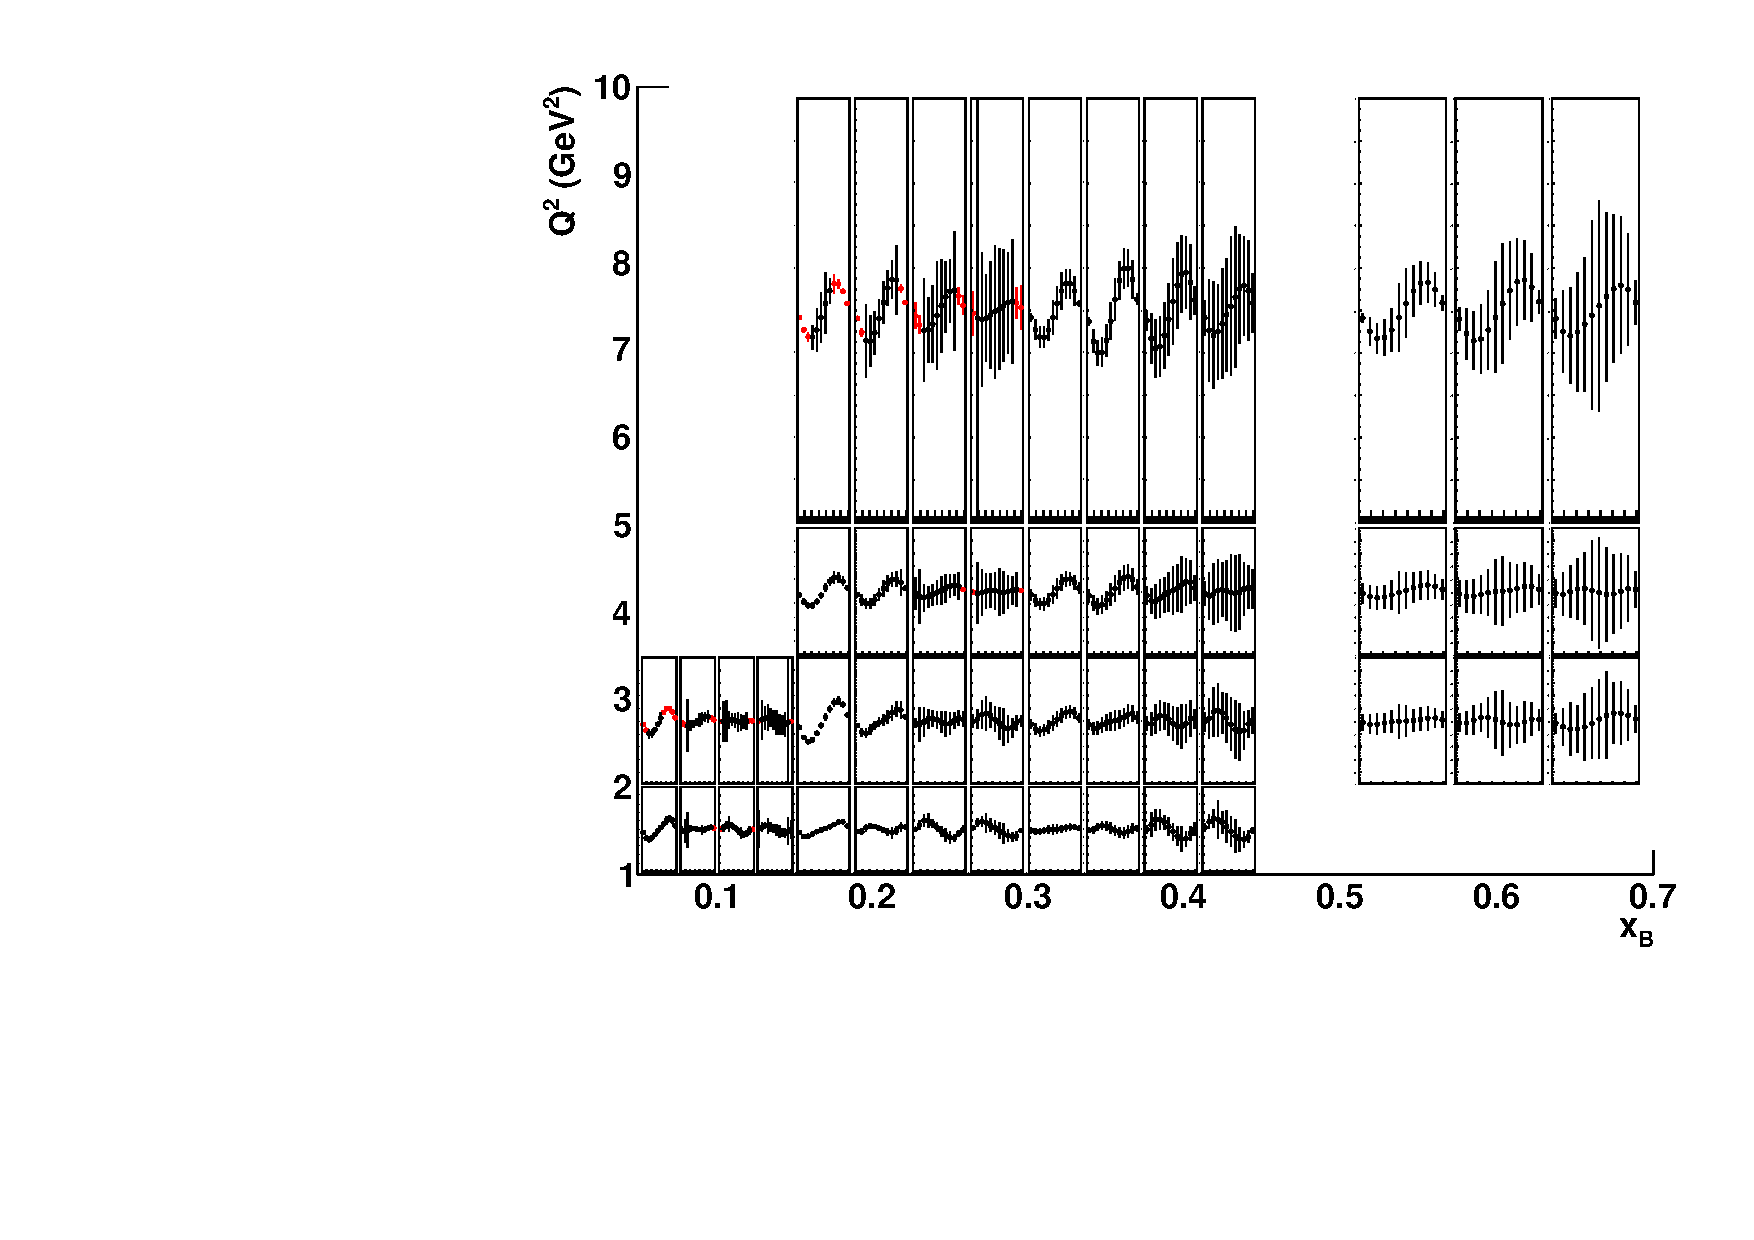
\includegraphics[width=200mm]{asym_polndvcs_tsa_newvgg_100days_FT_noFT.pdf}
%\caption[Projected target-spin asymetry]
%{Projected target-spin asymmetry. The y-scale range, common to all bins, is (-1;1). The black and red points are obtained, respectively, without and with the Forward Tagger. }\label{fig_tsa}
%\end{center}
%\end{sidewaysfigure}

\begin{sidewaysfigure}  
\begin{center}
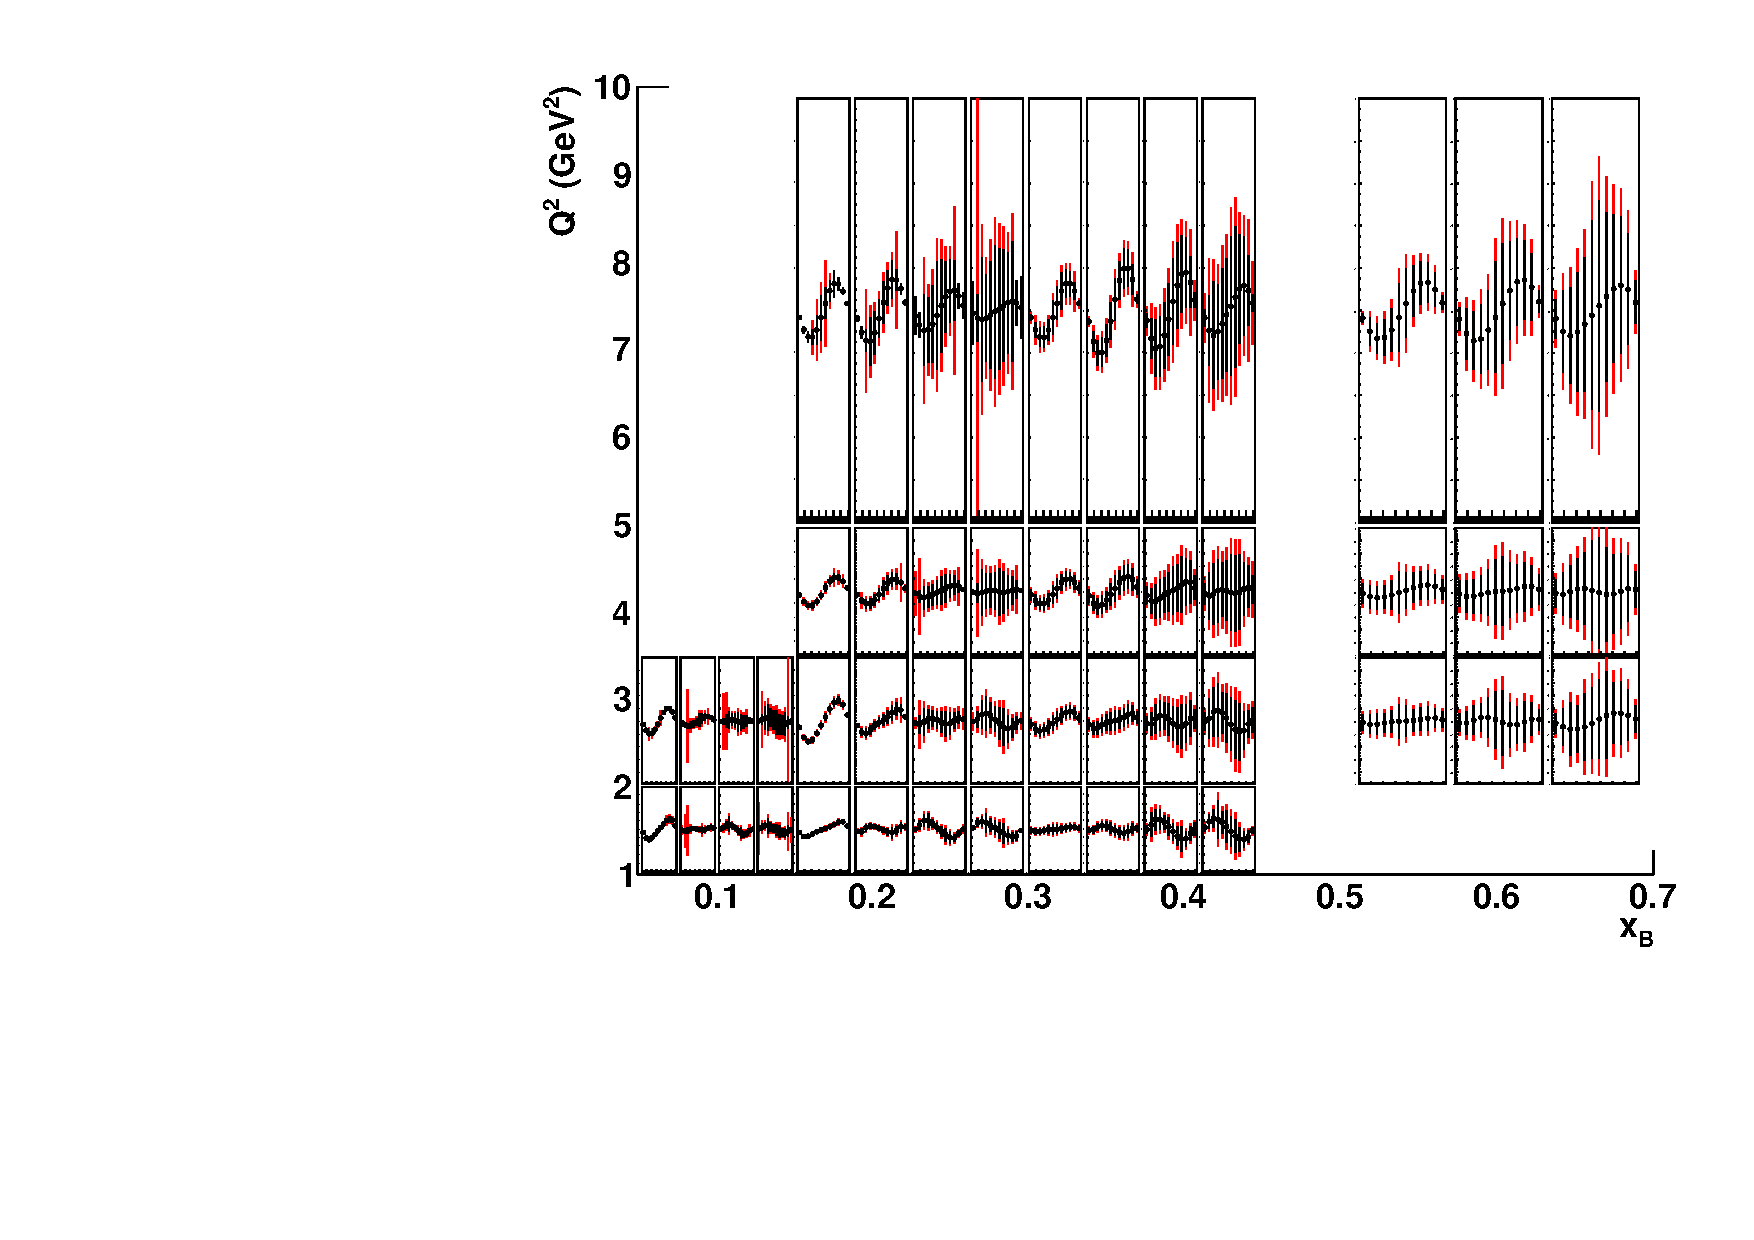
\includegraphics[width=200mm]{asym_polndvcs_tsa_newvgg_100_FT_and_noFT_50days.pdf}
\caption[Projected target-spin asymetry]
{Projected target-spin asymmetry. The y-scale range, common to all bins, is (-1;1). The black and red points are obtained, respectively, with 110 days and 50 days of beamtime.}\label{fig_tsa_100_50_FT}
\end{center}
\end{sidewaysfigure}

\begin{sidewaysfigure}  
\begin{center}
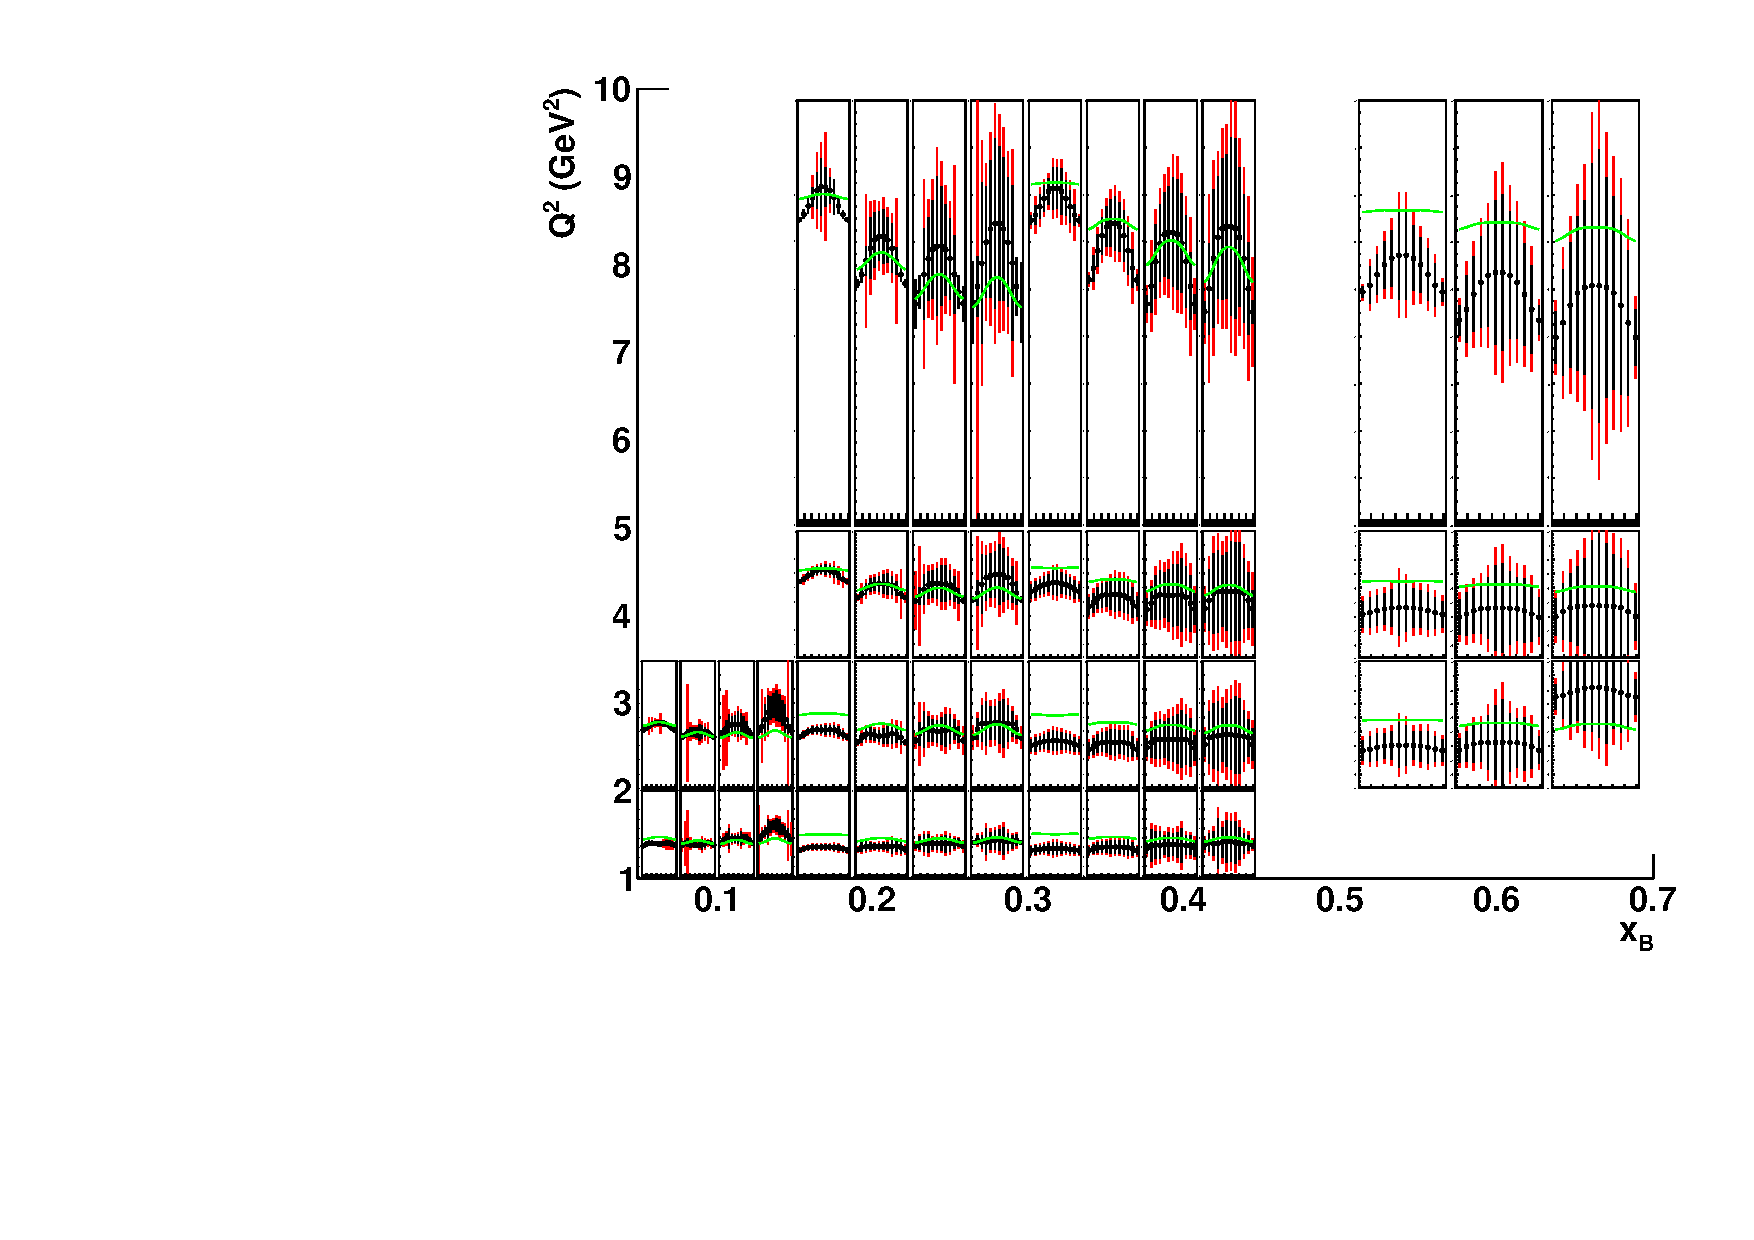
\includegraphics[width=200mm]{asym_polndvcs_dsa_newvgg_BH_100_50days_FT_and_noFT.pdf}
\caption[Projected double-spin asymmetry]
{Projected double-spin asymmetry, compared to the BH (green lines), calculated at the average kinematics of each bin. The y-scale range, common to all bins, is -0.6-1.2. The black and red points are obtained, respectively, with 110 days and 50 days of beamtime. }\label{fig_dsa_100_50_FT}
\end{center}
\end{sidewaysfigure}

\begin{sidewaysfigure}  
\begin{center}
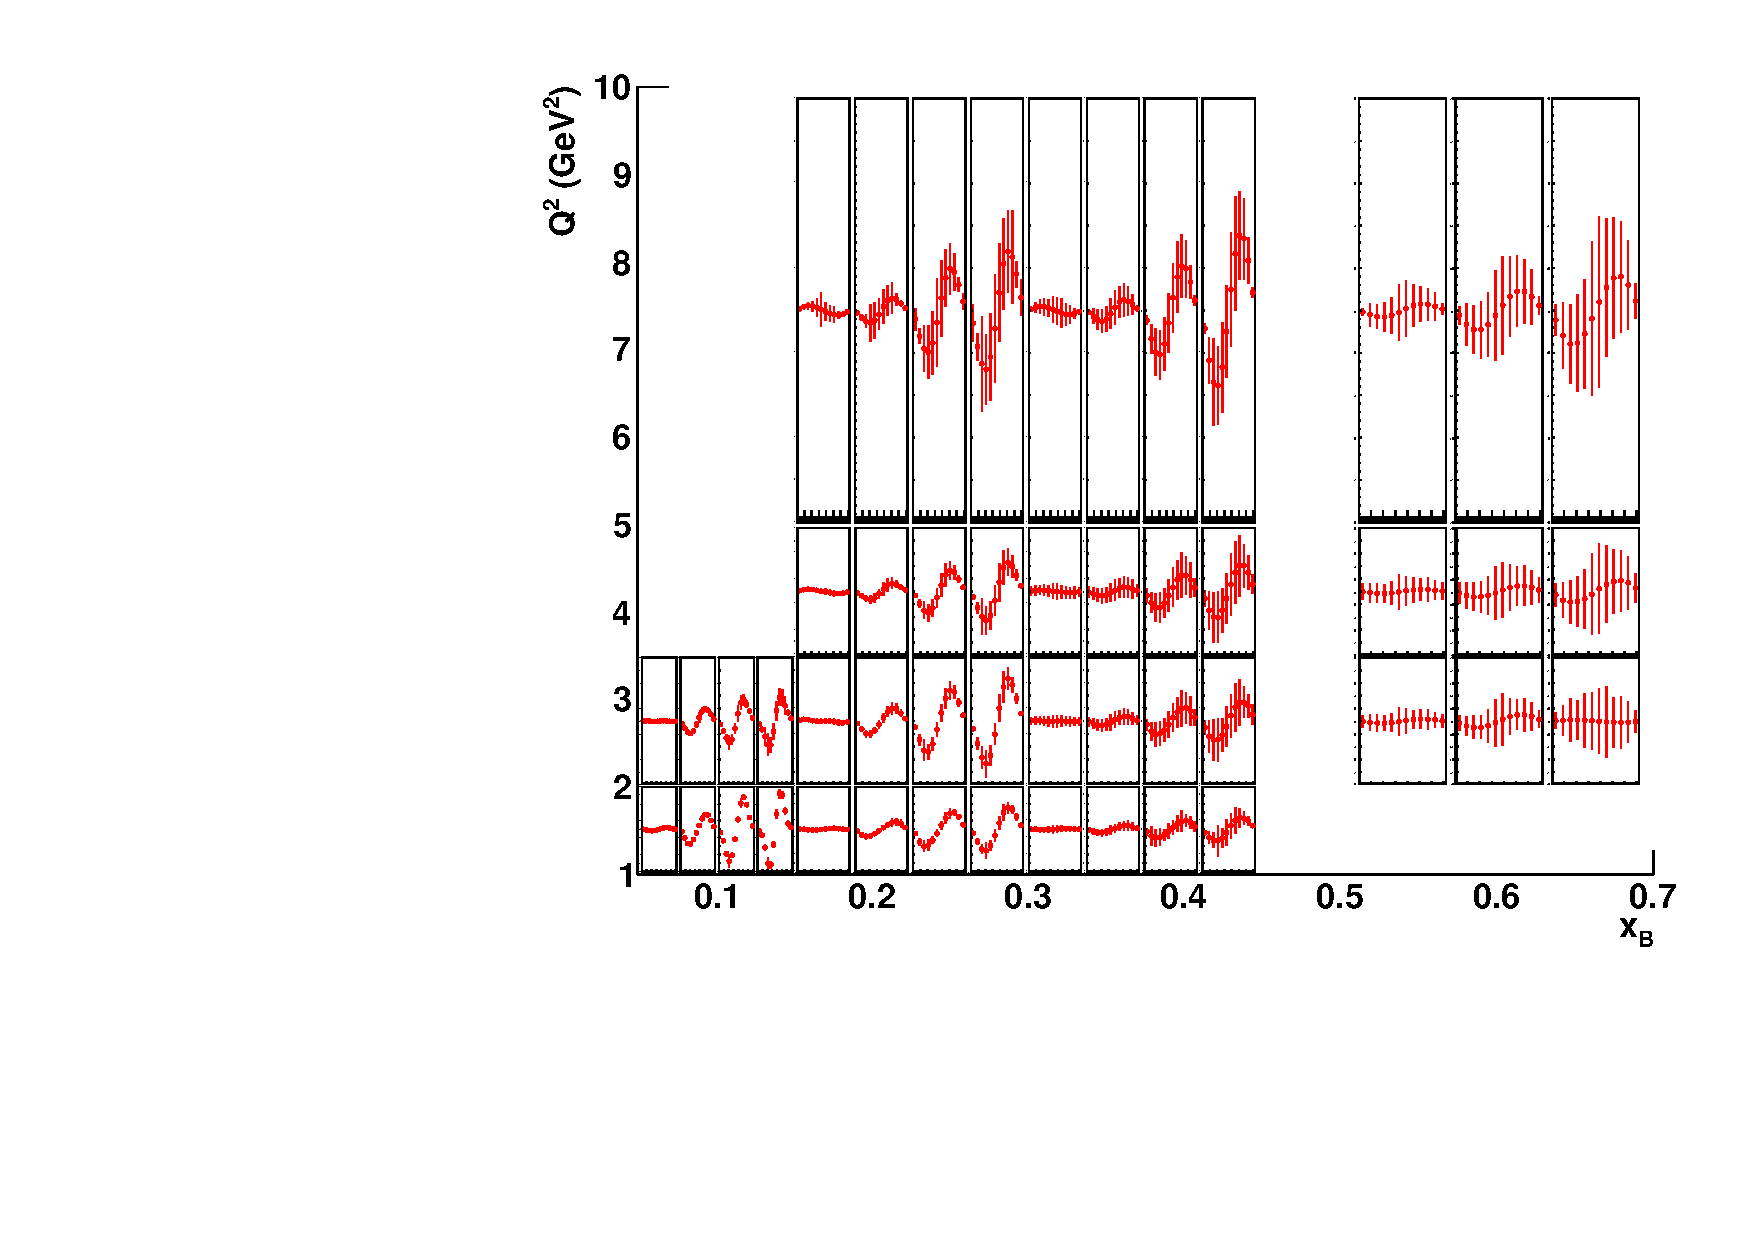
\includegraphics[width=160mm]{asym_newcuts_bsa_newvgg.pdf}
\caption[Projected beam-spin asymmetry from E12-11-003]
{Projected beam-spin asymmetry, as will be obtained from experiment E12-11-003 \cite{proposal}. The y-scale range, common to all bins, is -0.25-0.25.}\label{fig_bsa}
\end{center}
\end{sidewaysfigure}
